\documentclass[a4paper,12pt]{article}
\usepackage[hidelinks]{hyperref}
\usepackage{graphicx}
\usepackage{float}
\usepackage{caption}
\begin{document}
\begin{center}

%Cover page
\Huge\textbf{Testing Report\\}
																											
\vspace{2 cm}

\LARGE\textbf{Group Name:} Testing Status\newline
 
\vspace{0.5 cm}
\begin{tabular}{lr}
Daniel Christopher Alves Ara\"{u}jo&13073878\\ 
Taariq Ghoord&10132806\\
Lerato Molokomme&11197961\\
Semaka Malapane&13081129\\
Mpedi Mello&11210754\\
Ryno Pierce&12003922\\
Lutfiyya Razak&10198408\\
Frederick Snyman&13028741\\
Keagan Thompson&13023782\\
\end{tabular}

\vspace{1cm}
\textbf{Git repository link:\\}
\url{https://github.com/u13073878/COS301-Testing-Status}

\vspace{1cm}
\textbf{Date:} 24 April 2015
\end{center}
\pagenumbering{gobble}
\newpage

%table of contents
\tableofcontents
\pagenumbering{arabic}
\newpage

%github links 
%Group A - http://github.com/lana01/Status-A
%Group B - https://github.com/BuzzSpaceB/Status

%----------------1. Assess Profile ---------------
\section{assessProfile Use case}
\subsection{Group A - assessProfile}
%add test results for group A assessProfile here
%Lerato
Status A assesProfile function does not exists in the list of all the functions implemented. However the the function was used
inside the function ThreadsDepthAssessor which made it difficult to test. So the code fail to adhere to the specified pre-condition 
therefore  the post condition is also not met. ThreadsDepthAssesor was called and was used to test and the test failed.

\subsection{Group B - assessProfile}
%add test results for group B assessProfile here
%Mpedi
Status B provided the assessProfile function. However the parameter list was not done as specified in the master specifications. 
The assessProfile that was tested required 3 parameters (assessProfileRequest, user, callback) while the master specification 
specified only one parameter object that contains a profile ID. The assessProfile function did not test for the only pre-condition 
that was specified in the master specification, which is check if the profile with specified identity exists. So the code failed in 
that regard. In addition to that, it appears that the function did not do any profile assessment calculation at all, and thus gave 
the same response everytime it was ran. So the post-condition was not met. Status B assessProfile failed overall.


\newpage
%----------------2. Set status calculator ---------------
\section{setStatusCalculator Use case}
\subsection{Group A - setStatusCalculator}
%add test results for group A setStatusCalculator here
%Lutfiyya
Status A provided a setStatusCalculator. 
The setStatusCalculator function provided takes a setStatusCalculatorRequest which consists of the SpaceId and profileAssessorID.NumPostsAssessor and ProfileAssessor where implemented.
Nodeunit was used to test the setStatusCalculator function and the code of the unit test appears below:

\begin{figure}[H]
		\centering
		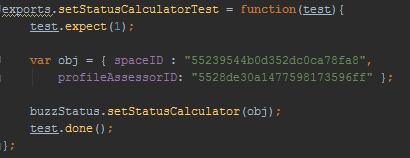
\includegraphics[width=1.0\textwidth]{Figures/setStatusCalculator.png}
		\caption{Unit tests for \textit{setStatusCalculator}}
	\end{figure}

Executing the tests above resulted in the following output:

	\begin{figure}[H]
		\centering
		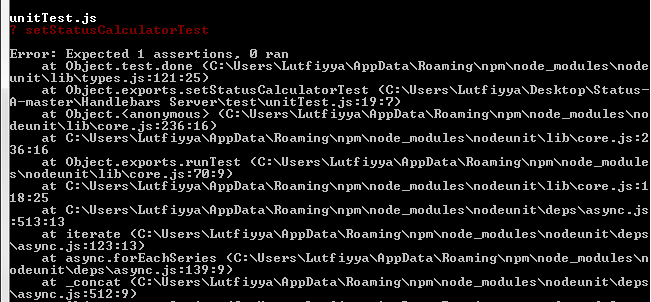
\includegraphics[width=1.0\textwidth]{Figures/setStatusCalculatorOutput.png}
		\caption{Results of the unit tests for \textit{setStatusCalculator}}
	\end{figure}
	
The test, setStatusCalculatorTest fails because ProfileAssessor function does not work. The pre-condition were not tested which was to test if a buzz space is open therefore the post-conditions were not met.

\subsection{Group B - setStatusCalculator}
%add test results for group B setStatusCalculator here
%Taariq
Status B did not implement all the status calculators. Only ThreadDepth and numPost assessors are provided. The numPostAssessor counts the threads of a particular user and sets that as the status level of the user. The threadDepthAssessor calculates a users status level based on an average calculated by number of threads divided by a count of the total threads of a user. Unit tests for this will follow.
It seems that the statusCalculatorRequest and statusCalculatorResult are implemented as functions so we cannot access their profileAssessors which must be the reason for the fail of the tests. Images are given below.

	\begin{figure}
		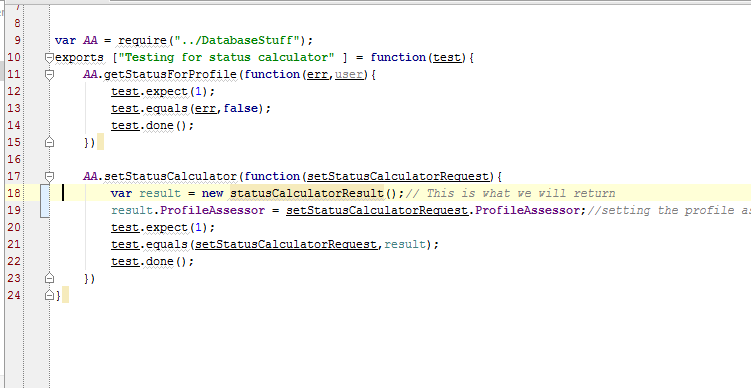
\includegraphics[width=1.0\textwidth]{Figures/codes.PNG}
		\caption{Unit tests for \textit{setStatusCalculator}}
	\end{figure}

	\begin{figure}
		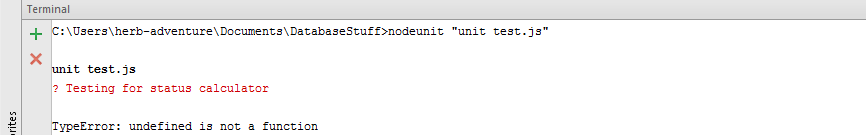
\includegraphics[width=1.0\textwidth]{Figures/statuscalculator.PNG}
		\caption{Unit tests for \textit{setStatusCalculator test output}}
	\end{figure}
	\begin{figure}
		
\includegraphics[width=1.0\textwidth]{Figures/statuscalculator2.PNG}
		\caption{Unit tests for \textit{setStatusCalculator test output}}
	\end{figure}

\newpage
%----------------3. Get status for profile ---------------
\section{getStatusForProfile Use case}
\subsection{Group A - getStatusForProfile}
%add test results for group A getStatusForProfile here
The function take the user ID and a callback. But the callback does not return and the user ID does not get initialized, hence the function is called on invalid parameters.
Pre-condition: user has an ID
Post-condition: User's profile is returned from the user ID.
	\begin{figure}
		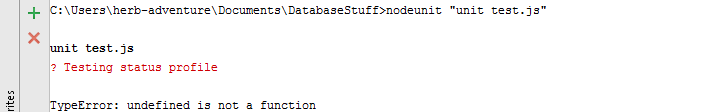
\includegraphics[width=1.0\textwidth]{Figures/get_status_profile.PNG}
		\caption{Unit tests for \textit{setStatusCalculator test output}}
	\end{figure}

	\begin{figure}
		
\includegraphics[width=1.0\textwidth]{Figures/get_status_profile2.PNG}
		\caption{Unit tests for \textit{setStatusCalculator test output}}
	\end{figure}



\subsection{Group B - getStatusForProfile}
%add test results for group B getStatusForProfile here
Status B provided a \textit{getStatusForProfile} as in Figure 41 of the master specifications. No pre- or post-conditions are tested for in the code written by Status B, however none were provided in the given master specifications.

The function that Status B provided takes as parameters the ID of the user being queried.

Nodeunit was used for doing unit tests on this code, and the code of the unit tests appears in the figure below:

	\begin{figure}[H]
		\centering
		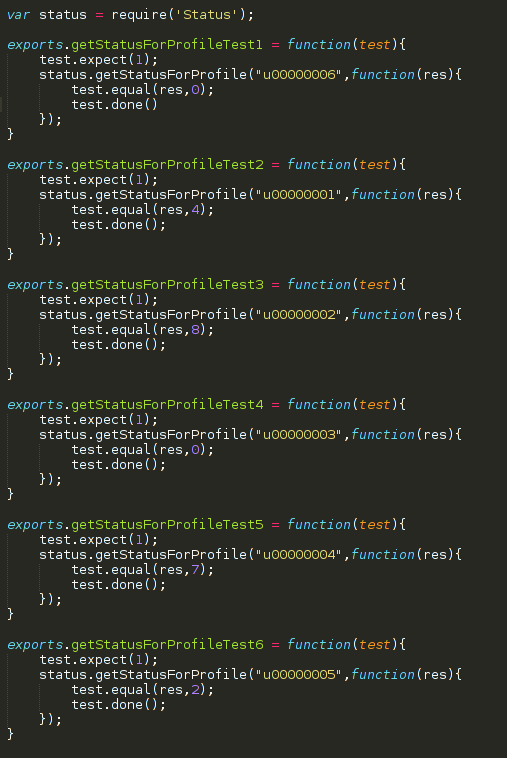
\includegraphics[width=1.0\textwidth]{Figures/getStatusForProfile_unittests.png}
		\caption{Unit tests for \textit{getStatusForProfile}}
	\end{figure}
	
Executing the tests above resulted in the following output:

	\begin{figure}[H]
		\centering
		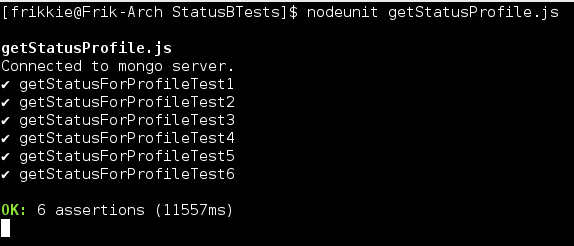
\includegraphics[width=1.0\textwidth]{Figures/getStatusForProfile_results.png}
		\caption{Results of the unit tests for \textit{getStatusForProfile}}
	\end{figure}
	
The tests that are run, checks the status value for six users present in the database, with differing status values. All six tests pass successfully and the function \textit{getStatusForProfile} appears to hav been implemented correctly as per the master specification. These test cases cover 100\% of the use cases as defined in the master specification.

\newpage
%----------------4. Create appraisal type ---------------
\section{createAppraisalType Use case}
\subsection{Group A - createAppraisalType}
%add test results for group A createAppraisalType here
%Keagan

As indicated in figure 43 of the master specification, Status A has met the requirements 
but I could not get the method to run in testing. If any null values are passed in, the code will not 
detect this problem which will cause the system to crash.

My testing code is given below:

 \begin{figure}[H]
 	\centering
 	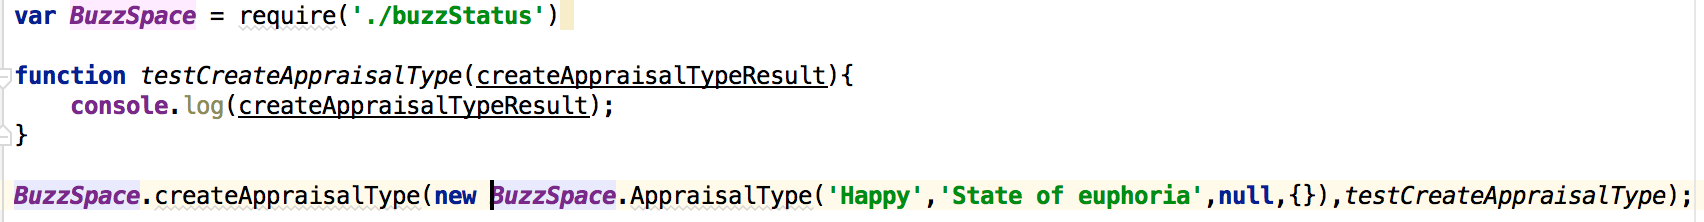
\includegraphics[width=1.0\textwidth]{Figures/KTCode.png}
 	\caption{Unit test for createAppraisalType}
 \end{figure}
 
 and the resulting code:
 
 \begin{figure}[H]
 	\centering
 	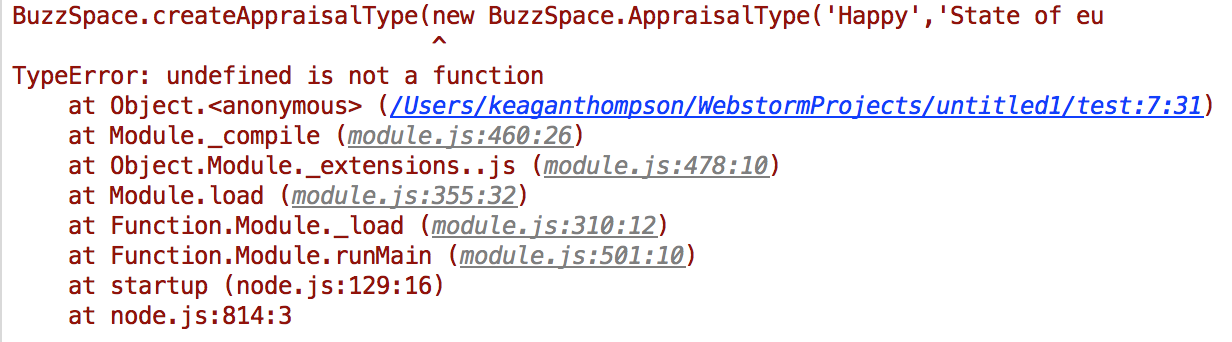
\includegraphics[width=1.0\textwidth]{Figures/KTError.png}
 	\caption{Unit test result for createAppraisalType}
 \end{figure}
 
 As the method was not runnable from my code, I looked at the code and could not see any code for verifying
 the database was working correctly or any other variables for that matter. The code looks confusing to run
 without any extra documentation.

\subsection{Group B - createAppraisalType}
%add test results for group B createAppraisalType here
%Semaka

The \textit{createAppraisalType} function created by Status B meets the requirements of the specification. The function implemented asks for the \textit{name} and \textit{description}. \textit{activityPeriod} is also created. Therefore the function meets the requirements as indicated in figure 43 of the specification.

The \textit{addAppraisalLevel} function created by Status B has a name and a level number. This meets the requirements.

The code for the unit tests is given below. The unit tests were made using Nodeunit.

\begin{figure}[H]
		\centering
		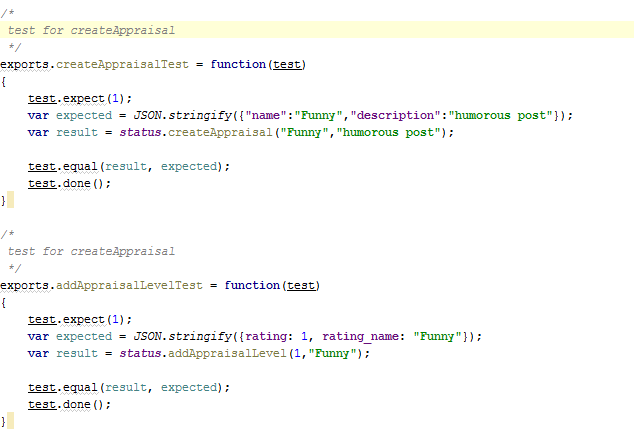
\includegraphics[width=1.0\textwidth]{Figures/createAppraisalTypeUnitTests.png}
		\caption{Unit test for createAppraisalType and addAppraisalLevel}
	\end{figure}

The following was the output of the createAppraisalType unit test created above:
\begin{figure}[H]
		\centering
		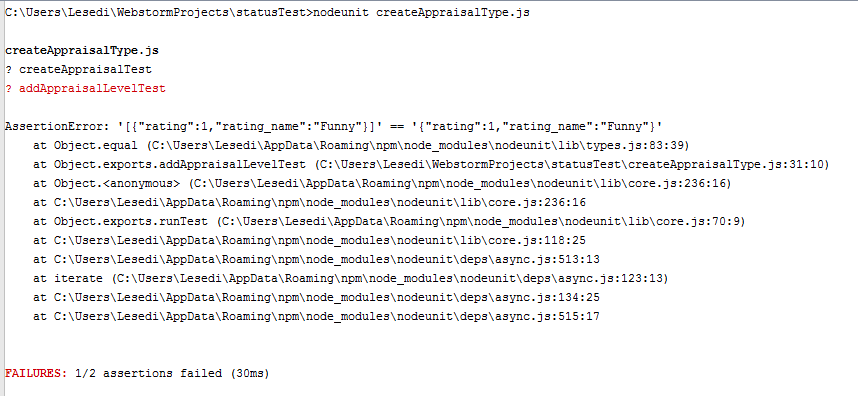
\includegraphics[width=1.0\textwidth]{Figures/createAppraisalTypeUnitTestsResult.png}
		\caption{The result of the unit test}
	\end{figure}
	
The \textit{createAppraisalType} function meets the post condition that an appraisal is created (the function passes the unit test) when the function is called.

The \textit{addAppraisalLevel} function doesn't meet the post condition, that is an appraisal level can't be created - the function fails the unit test.

\newpage
%----------------5. Activate appraisal type ---------------
\section{activateAppraisalType Use case}
\subsection{Group A - activateAppraisalType}
%add test results for group A activateAppraisalType here
%Ryno

Status A provides an \textit{activateAppraisalType} function, but does not match the specification. The function implemented asks for the \textit(appraisalType ID), but does not ask for a specific time period to be activated as indicated in figure 45 of the master specification. The code for the unit test is given by the figure below:


	\begin{figure}[H]
		\centering
		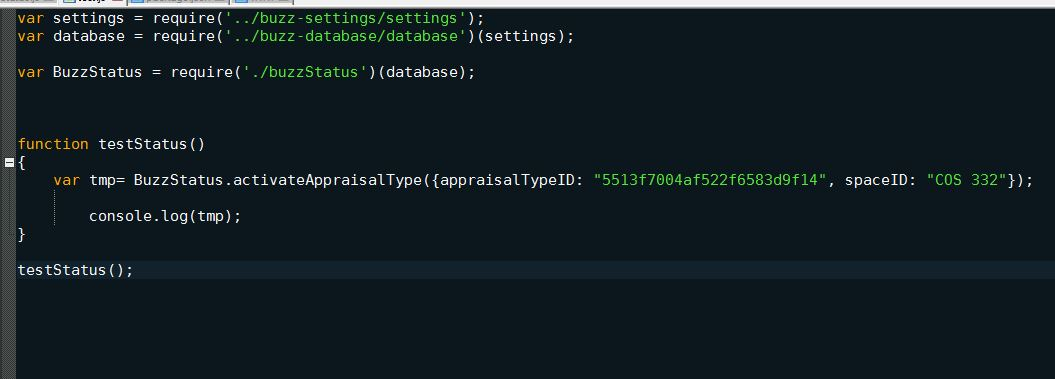
\includegraphics[width=1.0\textwidth]{Figures/activateTypeAtestcode.JPG}
		\caption{Unit test for activateAppraisalType}
	\end{figure}

The following is the result of running the code:

	\begin{figure}[H]
		\centering
		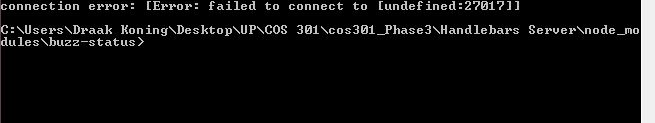
\includegraphics[width=0.8\textwidth]{Figures/activateTypeAResult.JPG}
		\caption{Output of unit tests for activateAppraisalType}
	\end{figure}

As you can see it could not connect to the database correctly in order to activate the appraisal type. Further inspection of the code show that it returns the value instead of using a callback function, this will cause it to always return empty or incorrect values as node runs asynchronously.

The implementation of the function does not meet the pre condition seeing that it doesn't test if the buzz space is active as well as, whether the active period is before the current date.

The post condition is net met due to the fact that the function could not connect to the database.

\subsection{Group B - activateAppraisalType}
%add test results for group B activateAppraisalType here
%Chris

Status B did not provide an explicit \textit{activateAppraisalType} function that matches Figure 45 of the project specifications.
However, Status B does provide two functions, \textit{activePeriod()} and \textit{setAppraisal()}.

The code for the unit tests is given by the figure below. For the test, NodeUnit was used.

	\begin{figure}[H]
		\centering
		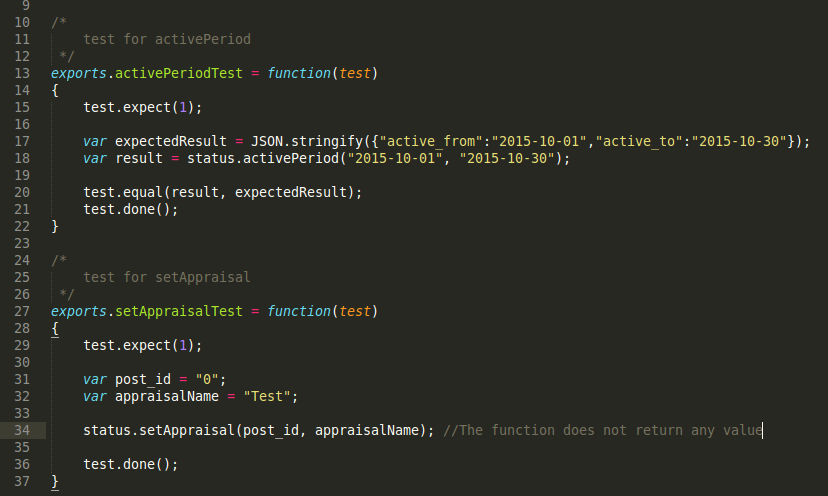
\includegraphics[width=1.0\textwidth]{Figures/activateAppraisalTypeUnitTests.png}
		\caption{Unit test for activateAppraisalType}
	\end{figure}

The following was the output given by NodeUnit.

	\begin{figure}[H]
		\centering
		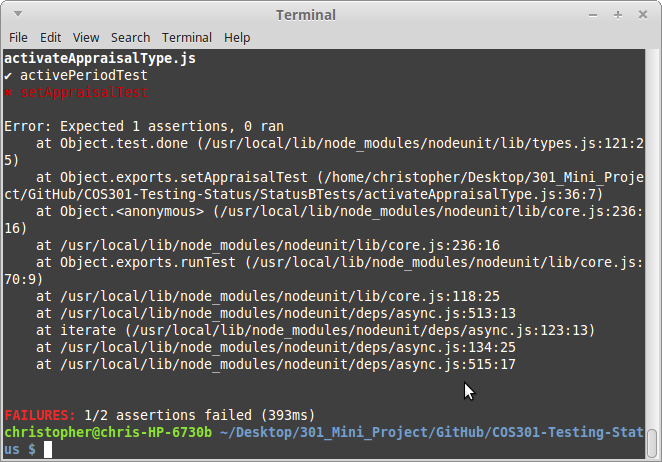
\includegraphics[width=0.8\textwidth]{Figures/activateAppraisalTypeUnitTestOutput.png}
		\caption{Output of unit tests for activateAppraisalType}
	\end{figure}

The first test, \textit{activePeriodTest}, passes. \textit{activePeriod()} takes two strings as parameters that represent the starting and ending date. However, it does no testing to ensure that the dates are in the correct format supported by JavaScript. Secondly, it does not have a callback parameter to specify a callback function, so it cannot be run asynchronously.

The section function, \textit{setAppraisal()}, fails. The function receives two parameters, a \textbf{post\_id} and and \textbf{appraisal\_name} to find a record in the database matching the \textbf{post\_id} and assign the \textbf{appraisal\_name} to \textbf{appraisal\_id} in the database. The function has an error that attempts to assign a null value to \textbf{post.appraisal\_id} in the database. 

The pre-conditions are not tested in either function, although a assumption can be made about a buzz space being active. However, \textit{setAppraisal()} does not test whether or not the active period is before the current date or time.

Due to the \textit{setAppraisal()} failing, the function does not meet the post-condition of appraisalTypeAssignment being persisted to the database.

\newpage
%----------------6 Assign appraisal to post ---------------
\section{assignAppraisalToPost Use case}
\subsection{Group A - assignAppraisalToPost}
%add test results for group A assignAppraisalToPost here
%Keagan and Ryno

Status A provides an \textit{assignAppraisalToPost} function that matches the spcification. The code for the unit test is given by the figure below:


	\begin{figure}[H]
		\centering
		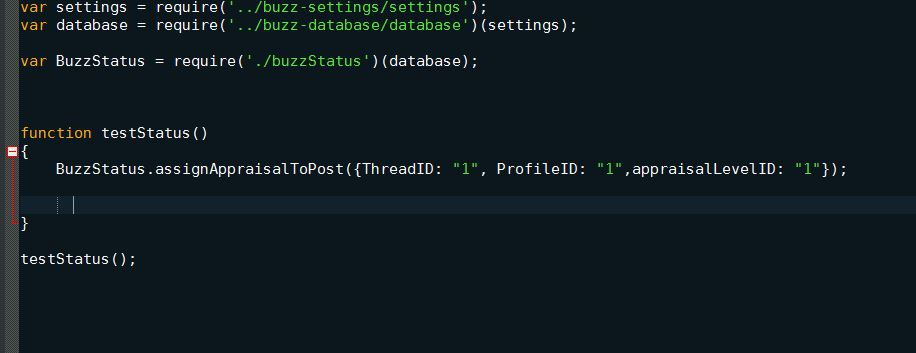
\includegraphics[width=1.0\textwidth]{Figures/aatptestCode.JPG}
		\caption{Unit test for activateAppraisalType}
	\end{figure}

The following is the result of running the code:

	\begin{figure}[H]
		\centering
		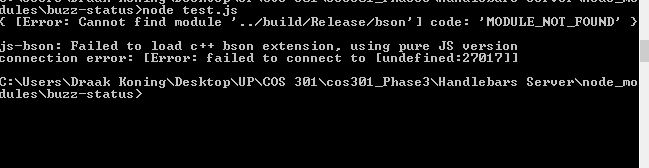
\includegraphics[width=0.8\textwidth]{Figures/aatpResult.JPG}
		\caption{Output of unit tests for assignAppraisalToPost}
	\end{figure}

As you can see it could not connect to the database to assign the appraisal. Further inspection of the code shows that the logic of the function is correct, unfortunately the pre condition is not tested to see if a buzz space is open. The post condition is not met as it couldn't assign the appraisal to a post.

\subsection{Group B - assignAppraisalToPost}
%add test results for group B assignAppraisalToPost here
%Frikkie
There is no explicit \textit{assignAppraisalToPost} function available from Status B, however, they have provided a function \textit{setAppraisal} which seems to attempt to fulfil that which is prescribed by \textit{assignAppraisalToPost}, as seen on Figure 46 of the master specifications.
The function \textit{setAppraisal} receives two parameters, the first is the post ID which is used to identify the post, and the second is the Appraisal ID, which is used to identify the ID that is to be assigned.

Nodeunit was used for doing the unit tests.

Below is the code for the unit tests that was used for testing \textit{setAppraisal}:

	\begin{figure}[H]
		\centering
		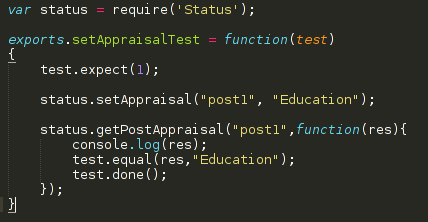
\includegraphics[width=0.8\textwidth]{Figures/assignAppraisalToPost_unittest.png}
		\caption{Unit tests for \textit{assignAppraisalToPost}}
	\end{figure}
	
The figure below is the result of running the unit tests


	\begin{figure}[H]
		\centering
		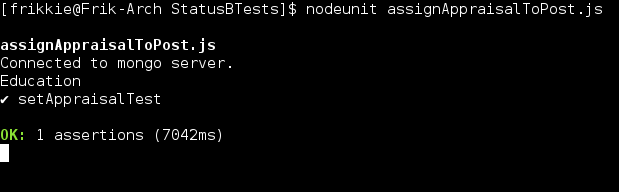
\includegraphics[width=0.8\textwidth]{Figures/assignAppraisalToPost_result.png}
		\caption{Results of the unit tests for \textit{assignAppraisalToPost}}
	\end{figure}

The pre-conditions to be held as per the master specifications, is that a buzz space must be open before the function \textit{assignAppraisalToPost} can be executed. It is not validated in the code that this pre-condition is upheld before continuing with execution. The post-condition hold, since the unit test passed.

The unit tests cover 100\% of the use cases.

\end{document}
